\section{Apparatus and Experiment}

\subsection{Basic Lowpass Filter Design}

Consider the first-order filter sketched in Figure~\ref{fig:RC}. The current $i$
over the capacitor is $i = C\frac{\dd v_c}{\dd t}$. Therefore, KVL around the
circuit gives 
%
\begin{equation}
    RC\frac{\dd v_c}{\dd t} + v_c = v_{\text{sig}} = A \cos{(\omega t)}
    \label{eq:de}
\end{equation} 
%
This differential equation has the transfer function \[ G(s) = \frac{1}
{RCs+1}. \] The steady-state solution of the differential equation~\eqref{eq:de}
is obtained as
%
\begin{align}
    \begin{split}
    v_c(t) &= A\abs{G(j \omega)}\cos{(\omega t + \angle G(j\omega))} \\
           &= \frac{A}{\sqrt{1+\omega^2R^2C^2}}\cos{\left(\omega t -
           \arctan{(\omega R C})\right)}
    \end{split}
    \label{eq:de_sol}
\end{align}
%
Since we do not want our signal to be attenuated by the low-pass filter, we must
choose the values of $R$ and $C$ such that $\omega R C \ll 1$ or $RC \ll
\nicefrac{1}{\omega}$. A difference of at least an order of magnitude should do
nicely.

\begin{figure}
\begin{circuitikz}[]
    \draw (0,0) to [vsource, l=$V_{\text{sig}}$] (0,3) to [R=$R$] (2,3) to
    [C=$C$] (2,0) -- (2,0) -- (0,0);

    \draw (2,3) to [short, *-o] ++(1,0) node[below]{$v_c$};
    \draw (2,0) to [short, *-o] ++(1,0);
    \node [ground] at (2,0) {};
\end{circuitikz}
\caption{An R-C low-pass filter circuit.}
\label{fig:RC}
\end{figure}

\subsection{Realistic Simulation}

We then perform a more realistic simulation with a second-order low-pass filter
with buffer connected to an amplifier op-amp with a gain of $3$. One of the
important aspects of this design is the selection of the op-amp. In order to
keep the common-mode voltage at $0$\unit{\volt} we choose the op-amps as CMOS
type. One such op-amp is the OP292~\todo{cite} and this op-amp is used in this
more realistic simulation.

The second order filter components are selected such that the resistances and
capacitances have the same value, satisfying the equation \[ f_c = \frac{1}{2\pi
RC}, \] where $f_c$ is the desired cutoff frequency of the filter, selected to
be a decade above the desired bioreactor oscillation at $90$\unit{\hertz}. We
respect the constraints $R \geq 1\unit{\kilo\ohm}$ and $C \geq
220\unit{\pico\farad}$. The values we used in the simulation were $R =
1\unit{\kilo\ohm}$ and $C = 0.1\unit{\micro\farad}$, yielding $f_c =
900\unit{\hertz}$.

The PWM signal generated by Teensy~\todo{cite} is simulated exactly
with a carrier frequency of $36.6$\unit{\kilo\hertz} modulating the signal \[
V_{\text{pwm}} = \nicefrac{3.3}{2} + \nicefrac{3.3}{2}\sin{(2\pi 90 t)}.\]
Finally, the impedance of the load (Physik Instrument (PI)
controller~\todo{cite}) is read off from its datasheet and inserted as a
$100$\unit{\kilo\ohm} resistance. The circuit that is simulated using
LTSpice~\todo{cite} is presented in Figure~\ref{fig:real_sig_gen}.

\begin{figure}[htb]
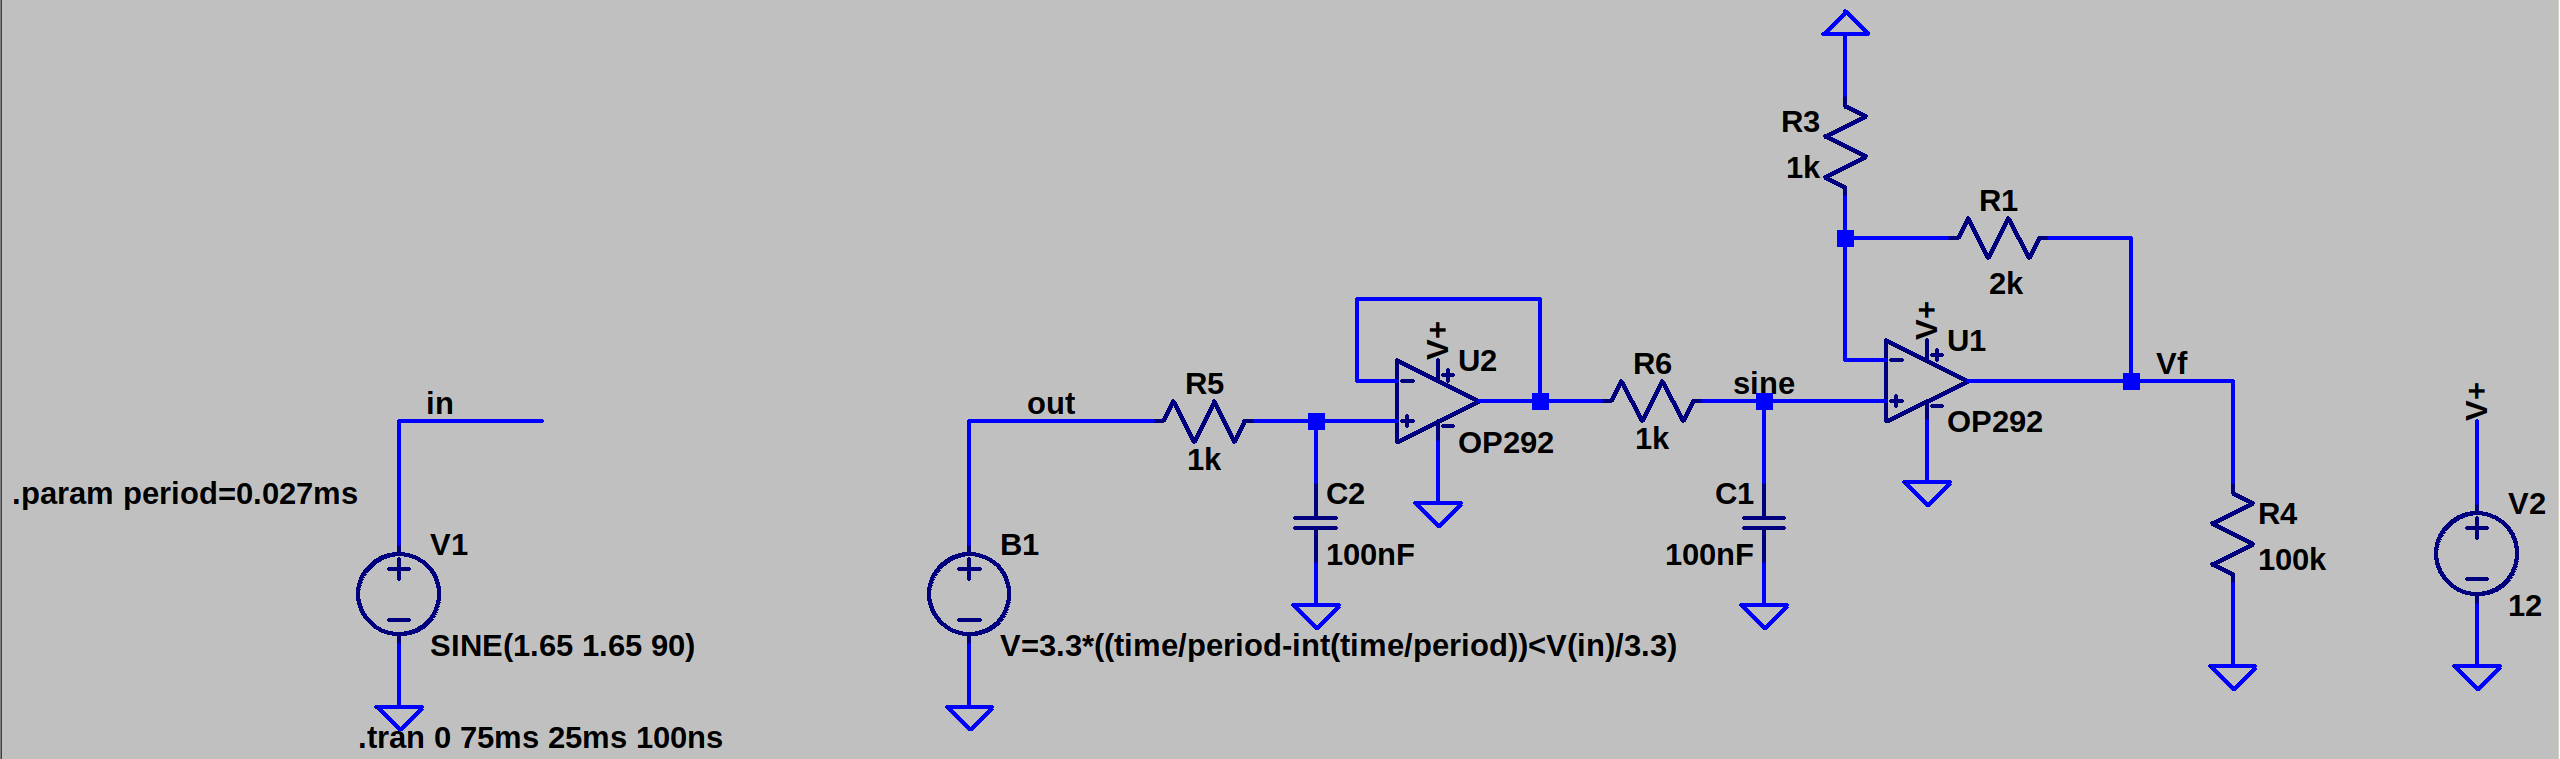
\includegraphics[width=8cm]{./figures/circuit.png}
\caption{The realistic signal generator circuit.}
\label{fig:real_sig_gen}
\end{figure}

The simulation generates the relevant voltage responses, provided in
Figure~\ref{fig:response}. The top plot shows the PWM signal generated by Teensy
modulating a sine-wave at $90$\unit{\hertz} frequency. The individual plots in
the middle show the output of the first (cyan) and the second (green) R-C
low-pass filters that extract the modulated signal from its PWM representation.
Finally, the last plot shows the amplified signal (gain: $3$) through the op-amp
OP292. This signal is ready to be sent to the PI controller.

\begin{figure}[t]
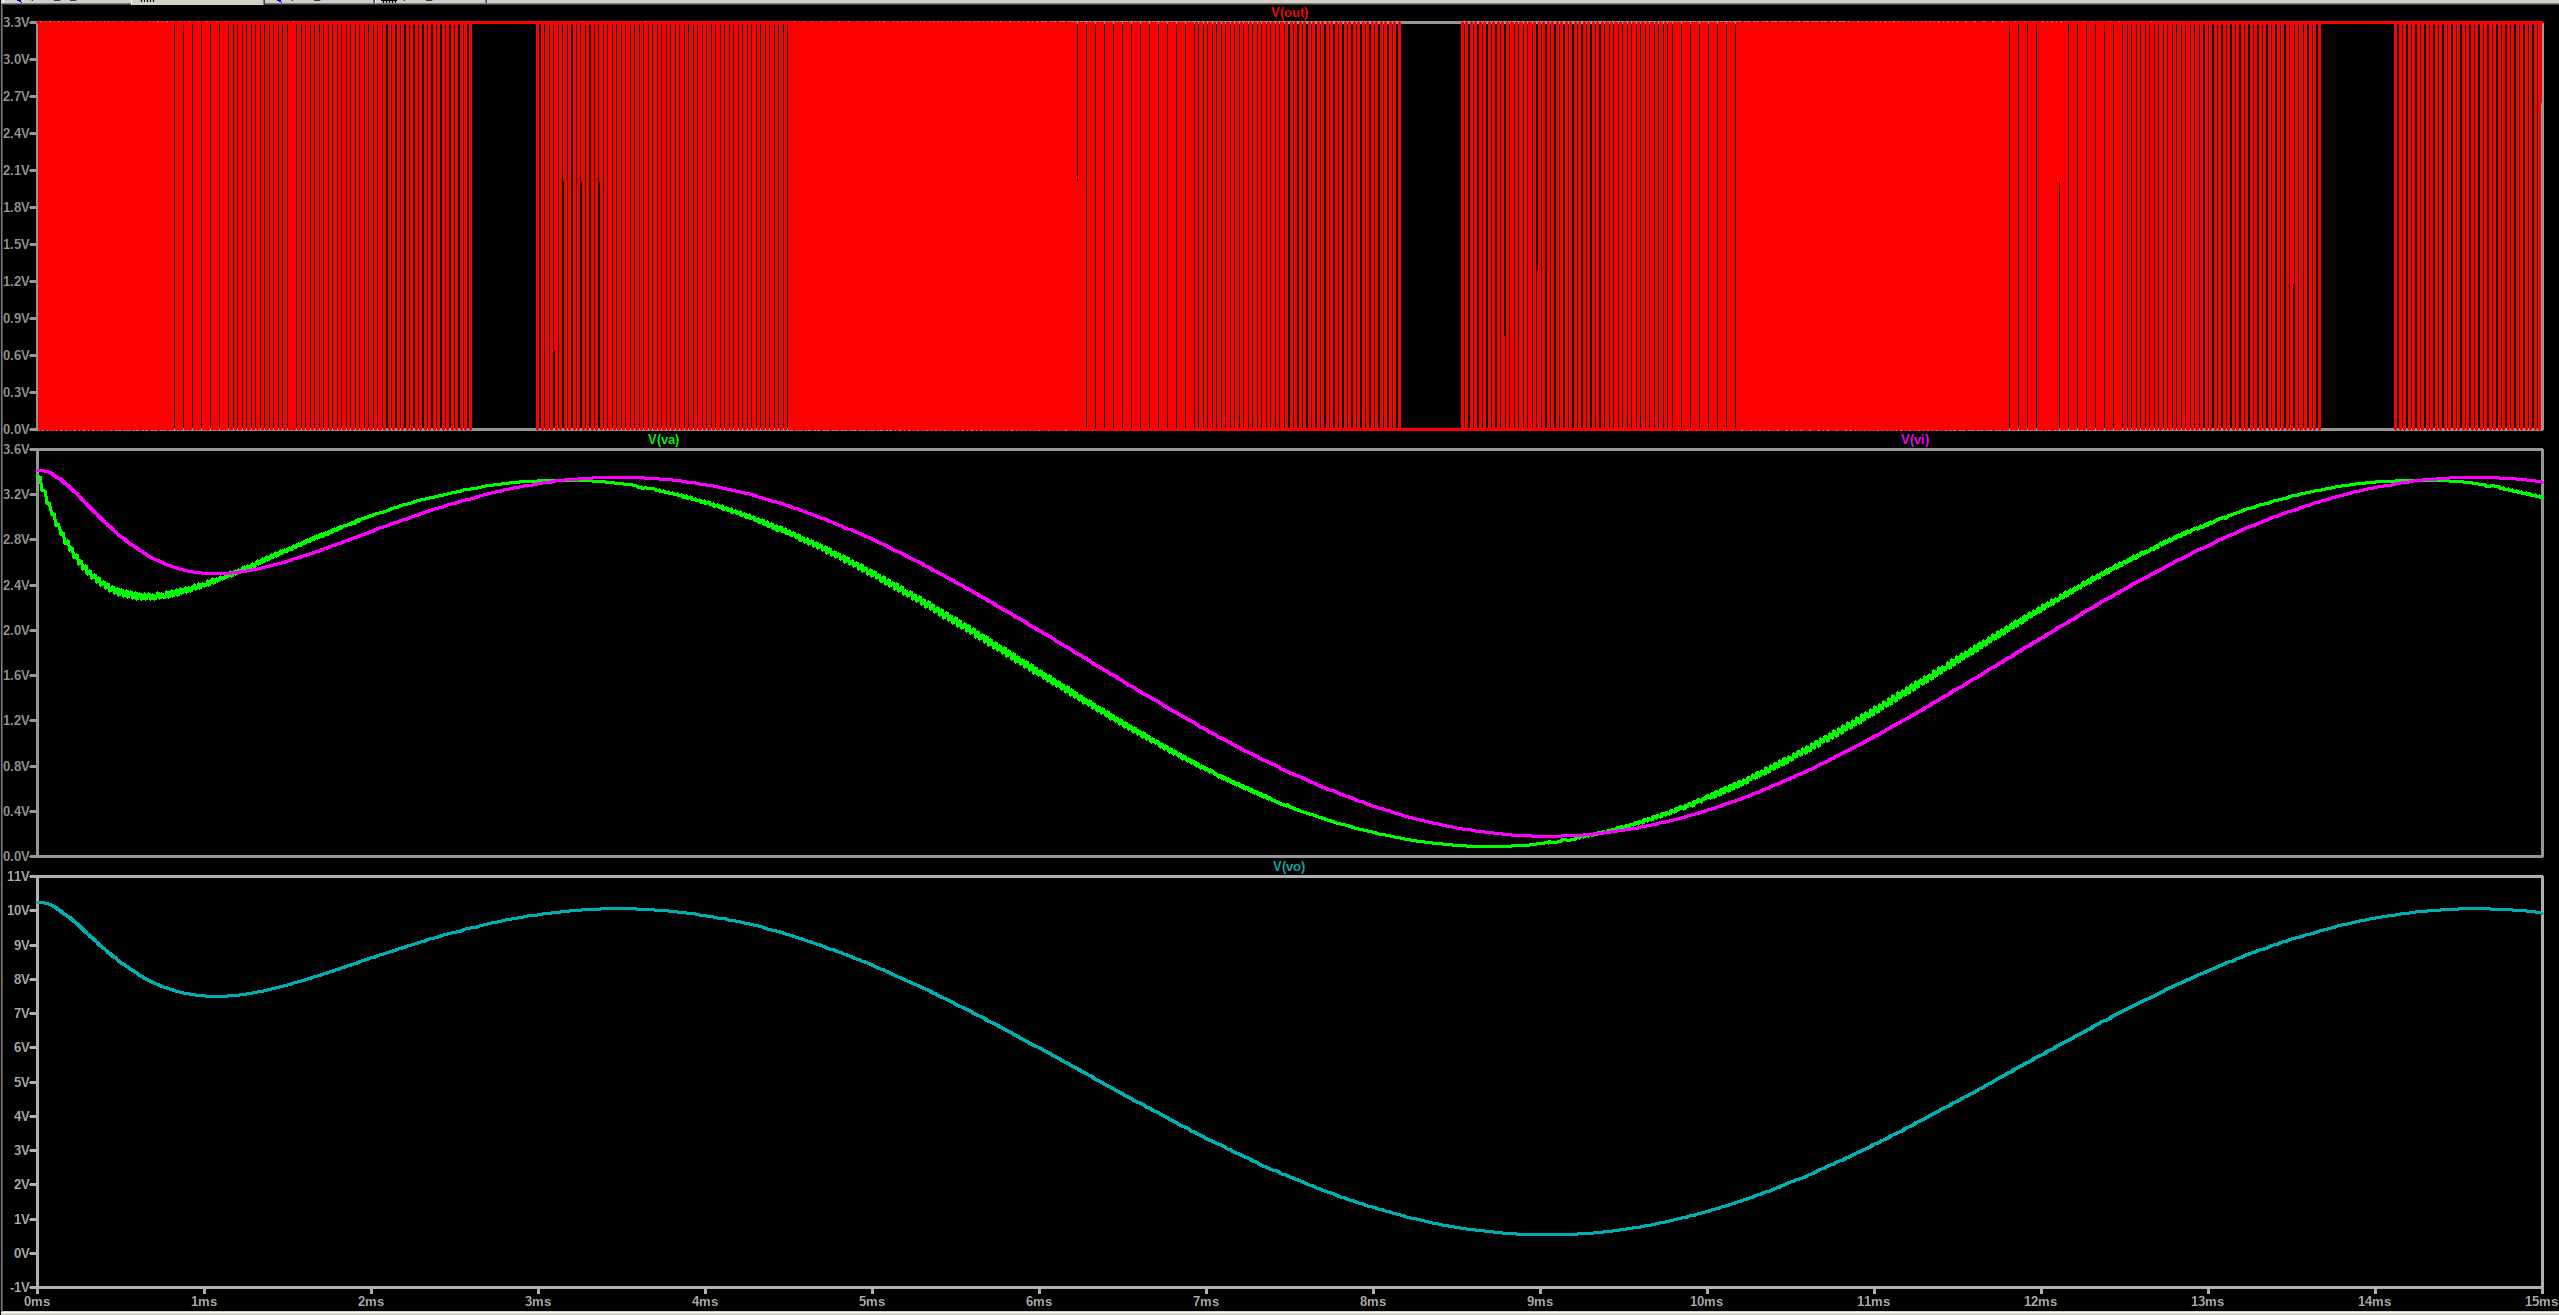
\includegraphics[width=0.5\textwidth]{./figures/pwm_filtered_one_two_final_signal.png}
\caption{The response of the realistic simulation.}
\label{fig:response}
\end{figure}
